\subsection{getDomainsByHostname}
Request Type: \textbf{POST}
\newline
Request Address: \textbf{/getdomainsbyhostname}
\newline

This endpoint takes in a JSON document containing a defined hostname with which to query all existing documents that contain this hostname in their "run\_information" field, if it exists. The returned data will also be a JSON document that contains all \textbf{unique} domain names found from documents containing the hostname.

It should be noted that only the documents uploaded using the Adapt uploader script found in ParFlow Performance Testing will have the "run\_information" embedded document field, so this will not return any document information taken from data uploaded using Shweta's uploader script.

\subsubsection{Data Format}
\textbf{Required Data}:
\newline
\newline
This endpoint takes in a JSON document in the request body using the format found in Figure \ref{fig:getdomainsbyhostname}. The "String" field should be replaced with the hostname being used to query.
\begin{figure}[h!]
    \centering
    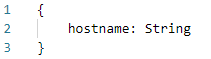
\includegraphics{img/getdomainsbyhostname.PNG}
    \caption{getDomainsByHostname Received Data Format}
    \label{fig:getdomainsbyhostname}
\end{figure}
\newline
\textbf{Returned Data}:
\newline
\newline
This endpoint will return a JSON document with a list containing all unique domains found in the database under the hostname provided. An example of what this JSON document looks like can be found in Figure \ref{fig:getdomainsbyhostname2}.

\begin{figure}[H]
    \centering
    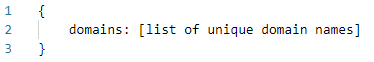
\includegraphics{img/getdomainsbyhostname2.PNG}
    \caption{getDomainsByHostname Returned Data Format}
    \label{fig:getdomainsbyhostname2}
\end{figure}

